\documentclass[pdf]{beamer}
\ProvidesPackage{preamble_slides}

% %% Beamer Stuff
\usetheme{Berlin}
\setbeamertemplate{footline}[frame number]
\setbeamertemplate{caption}[numbered]
\setbeamertemplate{section in toc}[sections numbered]
\setbeamertemplate{subsection in toc}[sections numbered]
\setbeamertemplate{navigation symbols}{} 
\setbeamercovered{transparent=25}
\usepackage{graphicx}
\usepackage{hhline}
\usepackage{appendixnumberbeamer}
\usepackage{multirow}
\definecolor{maincolor}{rgb}{0.6, 0.4, 0.7}
\usecolortheme[named = maincolor]{structure}
\renewcommand{\arraystretch}{1.5}

%% Bibliography packages
\usepackage{natbib}
\bibliographystyle{abbrvnat}

\title{Chinese Head Tax Project: Updates}
\author{Amy Kim}
\date{August 8, 2023}

\begin{document}
\begin{frame}[plain]
    \titlepage
\end{frame}

\begin{frame}{Research Question}
    How does an increase in fixed migration costs (in the form of a nationality-specific flat `head tax' at the time of entry) affect selection into immigration?
\end{frame}

% PART 1: IMMIGRATION INFLOW EFFECTS
\section{Immigration Inflow}
\begin{frame}[label = data1]
    \frametitle{Data Issues}
    \textbf{Ferenczi and Willcox (1929)}
    \begin{itemize}
        \item Immigration by country and year only starts in 1900 (no pre-period data for Head Tax)
        \item Census data is mostly similar in shape, but differs significantly at times \hyperlink{flow_compar_all}{\beamerbutton{All Countries}} \hyperlink{flow_compar_belgium}{\beamerbutton{Belgium}}  \hyperlink{flow_compar_japan}{\beamerbutton{Japan}}
    \end{itemize}
    \textbf{Time Series Emigration Regressions à la Hatton and Williamson (1994)}
    \begin{itemize}
        \item Essentially missing any origin country data for China (wages, population, industrialization)
        \item Don't have annual Chinese population in Canada -- okay to impute between decennial censuses?
    \end{itemize}
\end{frame}

\begin{frame}[label = flow_reg]
    \frametitle{Immigration Inflow: Regression Specification}
    \begin{multline}
        \text{FLOW}_t = \alpha + \beta_1\text{TOTALIMM}_t + \beta_2\text{GNPGROWTH}_t +  \\ \delta_1 t + \delta_2 t^2 + \sum_{\tau \in \mathcal{T}} \gamma^{FLOW}_\tau \mathbf{1}[TAX_t = \tau] 
    \end{multline}
    \begin{itemize}
        \item Same as regression from last time -- ctrls for total immigration, GNP growth, time and time squared; run separately for each country
    \end{itemize}
\end{frame}

\begin{frame}[label = country_regs]
    \frametitle{Graphing $\gamma^{FLOW}_\tau$'s for Various Countries [Eq (1)]}
    \begin{figure}
        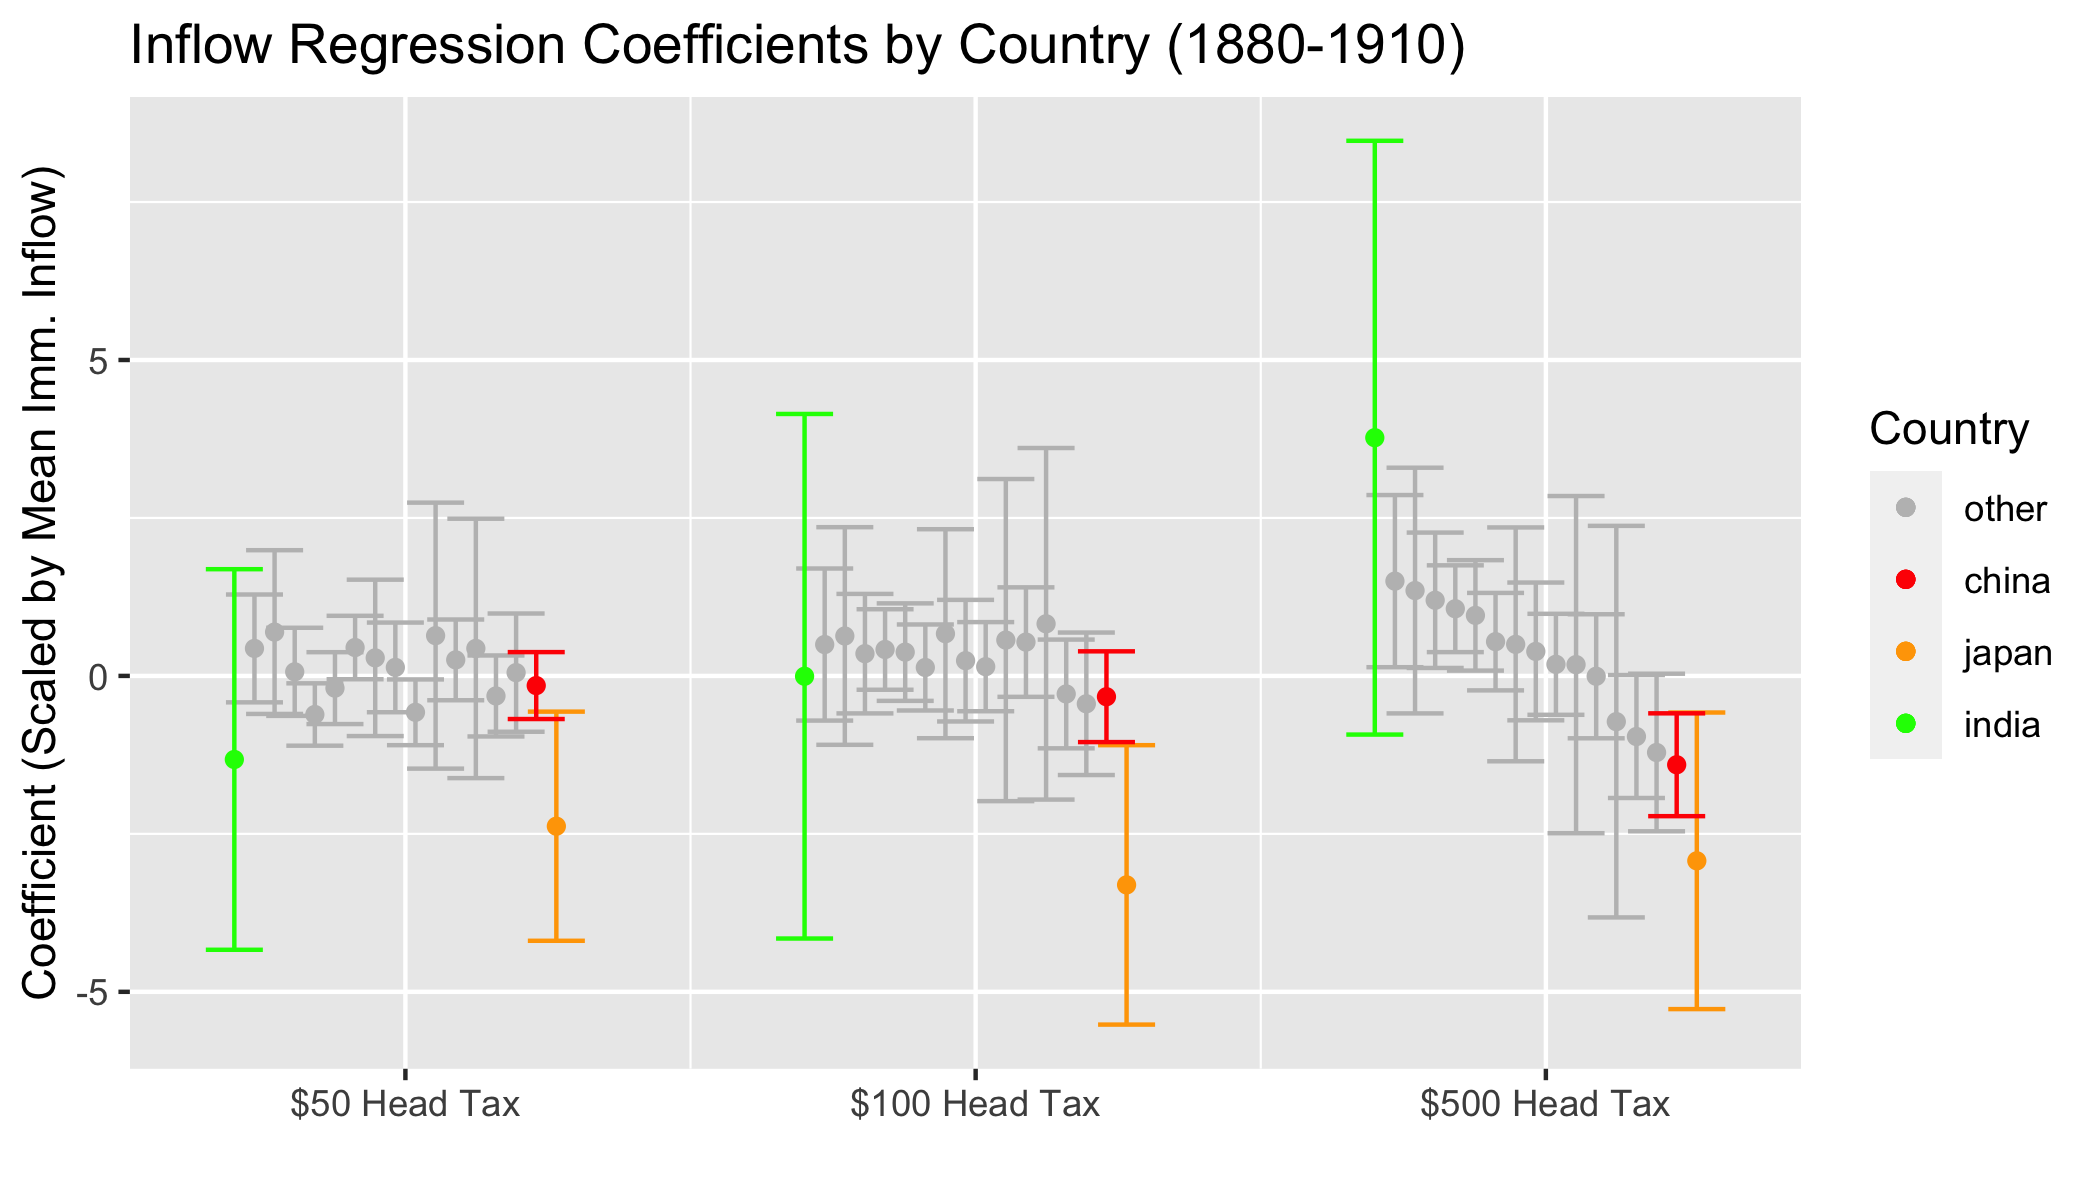
\includegraphics[width = \textwidth]{../../figs/8aug23/reg_coefs.png}
    \end{figure}
    \scriptsize
    Countries (L to R): India, Belgium, Australia/NZ, France, Poland, Russia, Italy, Denmark, Norway, Germany, Switzerland, Sweden, West Indies, Austria/Hungary, Finland, China, Japan
\end{frame}

% \begin{frame}[label = tab2_flow]
%     \frametitle{Immigration Inflow: Sig. Effects on Japanese Immigration?}
%     \centering
%     \begin{table}[H]
% 		\resizebox{\textwidth}{!}{
%             
% Table created by stargazer v.5.2.3 by Marek Hlavac, Social Policy Institute. E-mail: marek.hlavac at gmail.com
% Date and time: Mon, Jul 17, 2023 - 15:10:09
\begin{tabular}{@{\extracolsep{5pt}}lccccc} 
\\[-1.8ex]\hline 
\hline \\[-1.8ex] 
 & \multicolumn{5}{c}{\textit{Dependent variable:}} \\ 
\cline{2-6} 
\\[-1.8ex] & $CHIFLOW^R$ (Register) & $CHIFLOW^C$ (Census) & $JAPANFLOW^C$ (Census) & $CHIFLOW^C$ (Pre-1908) & $JAPANFLOW^C$ (Pre-1908) \\ 
\\[-1.8ex] & (1) & (2) & (3) & (4) & (5)\\ 
\hline \\[-1.8ex] 
 \$50 Tax &  & $-$453.700 & $-$383.200 & $-$96.840 & $-$56.450 \\ 
  &  & (399.800) & (242.300) & (294.200) & (187.600) \\ 
  & & & & & \\ 
 \$100 Tax & $-$695.100 & $-$599.000 & $-$867.000$^{**}$ & $-$283.200 & $-$1,089.000$^{***}$ \\ 
  & (834.500) & (604.800) & (366.500) & (353.100) & (225.100) \\ 
  & & & & & \\ 
 \$500 Tax & $-$6,989.000$^{***}$ & $-$1,607.000$^{**}$ & $-$810.100$^{*}$ & $-$1,188.000$^{**}$ & $-$1,620.000$^{***}$ \\ 
  & (1,006.000) & (669.300) & (405.600) & (471.200) & (300.500) \\ 
  & & & & & \\ 
\hline \\[-1.8ex] 
Observations & 38 & 41 & 41 & 28 & 28 \\ 
Adjusted R$^{2}$ & 0.747 & 0.675 & 0.430 & 0.730 & 0.833 \\ 
\hline 
\hline \\[-1.8ex] 
\textit{Note:}  & \multicolumn{5}{r}{$^{*}$p$<$0.1; $^{**}$p$<$0.05; $^{***}$p$<$0.01} \\ 
\end{tabular} 

% 		}
% 	\end{table}  
%     \hyperlink{census_flow}{\beamerbutton{Census Inflow w/ Japanese Imm.}}
% \end{frame}

% PART 2: IMMIGRANT COMPOSITION EFFECTS
\section{Immigrant Composition}
\begin{frame}[label = occ_n]
    \frametitle{Immigrant Composition: Profession at Arrival}
    \begin{figure}
        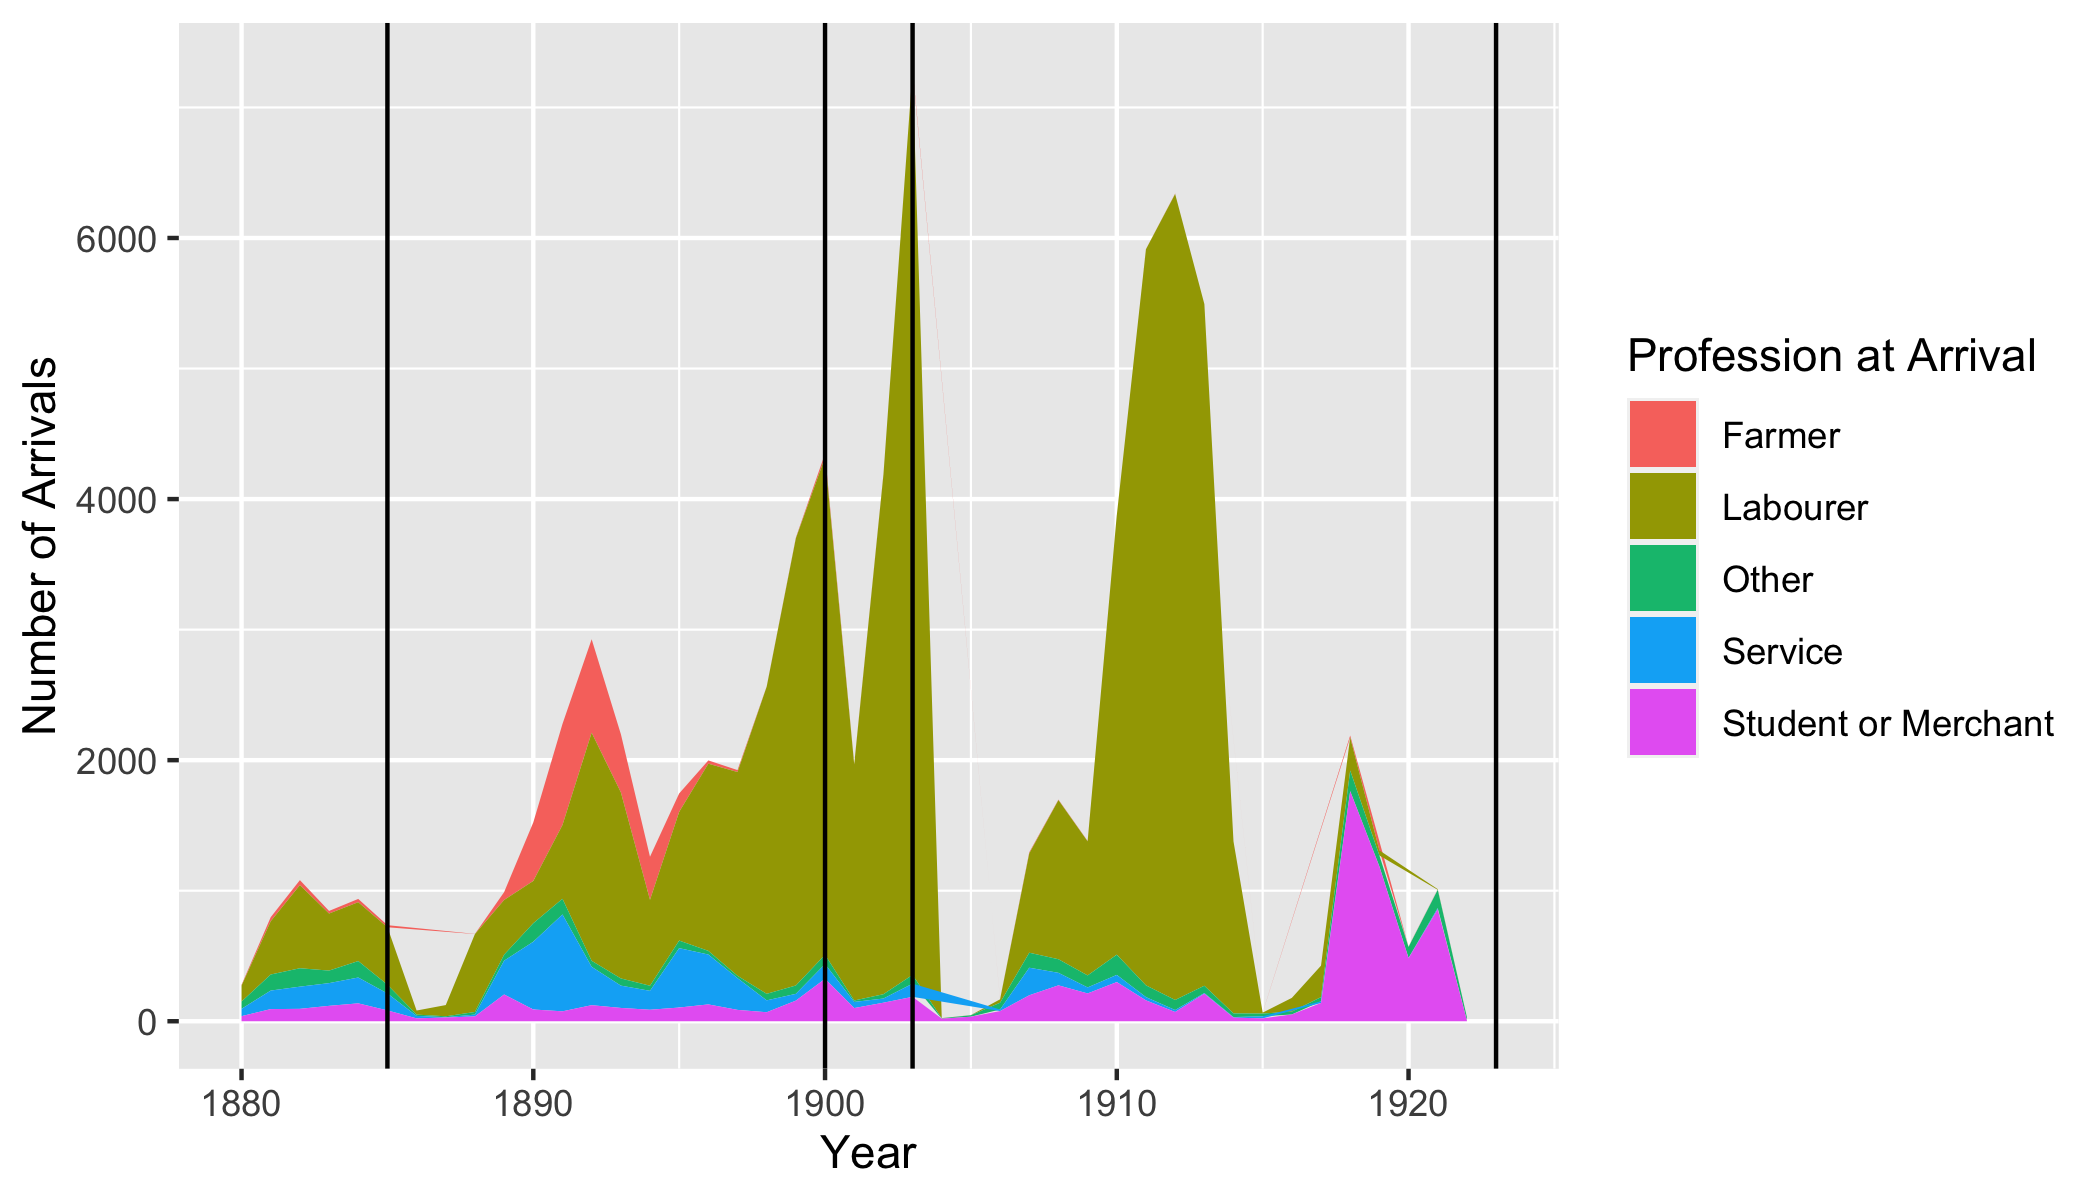
\includegraphics[width = \textwidth]{../../figs/8aug23/occgrp_n.png}
    \end{figure}
    \hyperlink{occ_pct}{\beamerbutton{As Percentages}}
\end{frame}

\begin{frame}[label = occ_n]
    \frametitle{Using Chinese Register Data}
    \begin{itemize}
        \item No comparison group -- hard to distinguish between time trends and effects of Head Tax 
        \item Regression specification: controlling for age and time trend only
        \item Exclude non tax payers (mechanically positively selected) and pre-1885 arrivals (also potential selection into registration)
        \item Results seem to support positive selection in higher head-tax years 
    \end{itemize}
\end{frame}

\begin{frame}[label = register_regs]
	\frametitle{Immigrant Composition Regressions: Register Data}
    \centering
    \begin{table}[H]
		\resizebox{0.65\textwidth}{!}{
            
% Table created by stargazer v.5.2.3 by Marek Hlavac, Social Policy Institute. E-mail: marek.hlavac at gmail.com
% Date and time: Tue, Aug 08, 2023 - 14:24:45
\begin{tabular}{@{\extracolsep{5pt}}lcc} 
\\[-1.8ex]\hline 
\hline \\[-1.8ex] 
\\[-1.8ex] & LABOR & HEIGHT \\ 
\\[-1.8ex] & (1) & (2)\\ 
\hline \\[-1.8ex] 
 \$100 Tax & $-$0.094$^{***}$ (0.006) & 0.052 (0.033) \\ 
  \$500 Tax & $-$0.482$^{***}$ (0.009) & 0.147$^{***}$ (0.055) \\ 
 Dep. Var. Mean & 0.748 (0.002) & 64.21 (0.009) \\ 
\hline \\[-1.8ex] 
Observations & 48,084 & 47,266 \\ 
Adjusted R$^{2}$ & 0.210 & 0.012 \\ 
\hline \\[-1.8ex] 
\end{tabular} 

		}
	\end{table} 
    \hyperlink{register_labor}{\beamerbutton{\% Laborer Over Time}} 
    \hyperlink{register_height}{\beamerbutton{Avg. Height Over Time}}
\end{frame}

\begin{frame}[label = reg_spec]
    \frametitle{Immigrant Composition: Regression Specification}
    \centering
    \begin{multline}
        y_{itc} = \beta_a AGE_{ic} + \delta_c + \delta_t + \alpha CHI_i + \\ \sum_{\tau \in \{100,500\}} \gamma_{\tau} CHI_i \times \mathbf{1}[TAX_t = \tau] + \varepsilon_{it}
    \end{multline}
    \begin{itemize}
        \item $\delta_c$ absorbs census year FE, $\delta_t$ absorbs arrival year FE
        \item controls for current age $AGE_{ic}$
        \item comparison group: all other immigrants
    \end{itemize}
\end{frame}

\begin{frame}[label = reg_can]
	\frametitle{Outcome Regressions: Canada (1880-1910)}
    \centering
    \begin{table}[H]
		\resizebox{\textwidth}{!}{
            
% Table created by stargazer v.5.2.3 by Marek Hlavac, Social Policy Institute. E-mail: marek.hlavac at gmail.com
% Date and time: Tue, Aug 08, 2023 - 13:13:55
\begin{tabular}{@{\extracolsep{5pt}}lcccc} 
\\[-1.8ex]\hline 
\hline \\[-1.8ex] 
\\[-1.8ex] & LABOR & CANREAD & EARN & HOUSEOWN \\ 
\\[-1.8ex] & (1) & (2) & (3) & (4)\\ 
\hline \\[-1.8ex] 
 $BORNCHI$ & 0.215$^{***}$ (0.026) & $-$0.324$^{***}$ (0.020) & $-$530.000$^{***}$ (107.100) & $-$0.463$^{***}$ (0.032) \\ 
  $BORNCHI \times$ \$50 Tax & $-$0.049$^{*}$ (0.029) & 0.107$^{***}$ (0.021) & 169.500 (117.300) & 0.109$^{***}$ (0.035) \\ 
  $BORNCHI \times$ \$100 Tax & 0.017 (0.032) & 0.113$^{***}$ (0.023) & 81.170 (133.200) & 0.071$^{*}$ (0.039) \\ 
  $BORNCHI \times$ \$500 Tax & $-$0.116$^{***}$ (0.029) & 0.074$^{***}$ (0.021) & 126.100 (119.500) & 0.126$^{***}$ (0.035) \\ 
 Dep. Var. Mean (SE) & 0.207 (0.002) & 0.923 (0.001) & 800.5 (6.515) & 0.473 (0.002) \\ 
\hline \\[-1.8ex] 
Observations & 63,181 & 62,059 & 38,073 & 63,181 \\ 
Adjusted R$^{2}$ & 0.048 & 0.053 & 0.047 & 0.140 \\ 
\hline \\[-1.8ex] 
\end{tabular} 

		}
	\end{table}  
\end{frame}

\begin{frame}[label = reg_us]
	\frametitle{Outcome Regressions: US (1880-1910)}
    \centering
    \begin{table}[H]
		\resizebox{\textwidth}{!}{
            
% Table created by stargazer v.5.2.3 by Marek Hlavac, Social Policy Institute. E-mail: marek.hlavac at gmail.com
% Date and time: Tue, Aug 08, 2023 - 14:55:16
\begin{tabular}{@{\extracolsep{5pt}}lcccc} 
\\[-1.8ex]\hline 
\hline \\[-1.8ex] 
\\[-1.8ex] & LABOR & CANREAD & ERSCORE & HOUSEOWN \\ 
\\[-1.8ex] & (1) & (2) & (3) & (4)\\ 
\hline \\[-1.8ex] 
 $BORNCHI$ & 0.022$^{***}$ (0.002) & $-$0.157$^{***}$ (0.001) & $-$14.680$^{***}$ (0.117) & $-$0.377$^{***}$ (0.002) \\ 
  $BORNCHI \times$ \$50 Tax & $-$0.075$^{***}$ (0.003) & 0.056$^{***}$ (0.002) & $-$2.437$^{***}$ (0.171) & 0.105$^{***}$ (0.003) \\ 
  $BORNCHI \times$ \$100 Tax & $-$0.167$^{***}$ (0.007) & 0.115$^{***}$ (0.006) & $-$0.341 (0.470) & 0.158$^{***}$ (0.008) \\ 
  $BORNCHI \times$ \$500 Tax & $-$0.246$^{***}$ (0.004) & 0.182$^{***}$ (0.003) & 1.612$^{***}$ (0.270) & 0.236$^{***}$ (0.005) \\ 
 Dep. Var. Mean (SE) & 0.219 (0.000) & 0.884 (0.000) & 48.3 (0.007) & 0.332 (0.000) \\ 
\hline \\[-1.8ex] 
Observations & 14,169,366 & 14,169,366 & 13,020,671 & 14,169,366 \\ 
Adjusted R$^{2}$ & 0.042 & 0.039 & 0.013 & 0.086 \\ 
\hline \\[-1.8ex] 
\end{tabular} 

		}
	\end{table}  
    \hyperlink{flow_us_can}{\beamerbutton{US/Canada Imm. Inflows}}
\end{frame}



% \begin{frame}[label = tab3_new_canread]
% 	\frametitle{Outcome Regressions: CANREAD}
%     \centering
%     \begin{table}[H]
% 		\resizebox{\textwidth}{!}{
%             
% Table created by stargazer v.5.2.3 by Marek Hlavac, Social Policy Institute. E-mail: marek.hlavac at gmail.com
% Date and time: Thu, Jul 20, 2023 - 16:52:44
\begin{tabular}{@{\extracolsep{5pt}}lcccccc} 
\\[-1.8ex]\hline 
\hline \\[-1.8ex] 
 & All (1890-1920) & All (1870-1920) & All (All Census Yrs) & Japan. (1890-1908) & Japan. (1870-1908) & Japan. (All Census Yrs) \\ 
\\[-1.8ex] & (1) & (2) & (3) & (4) & (5) & (6)\\ 
\hline \\[-1.8ex] 
 $BORNCHI$ & $-$0.305$^{***}$ & $-$0.313$^{***}$ & $-$0.344$^{***}$ & $-$0.147$^{***}$ & $-$0.445$^{*}$ & $-$0.292 \\ 
  & (0.018) & (0.027) & (0.018) & (0.052) & (0.266) & (0.208) \\ 
  & & & & & & \\ 
 $BORNCHI \times$ \$50 Tax &  & 0.016 & 0.128$^{***}$ &  & 0.323 & 0.308 \\ 
  &  & (0.032) & (0.020) &  & (0.271) & (0.210) \\ 
  & & & & & & \\ 
 $BORNCHI \times$ \$100 Tax & 0.146$^{***}$ & 0.154$^{***}$ & 0.134$^{***}$ & 0.384$^{***}$ & 0.682$^{**}$ & 0.365$^{*}$ \\ 
  & (0.026) & (0.033) & (0.022) & (0.095) & (0.278) & (0.217) \\ 
  & & & & & & \\ 
 $BORNCHI \times$ \$500 Tax & 0.030 & 0.037 & 0.081$^{***}$ & 0.076 & 0.374 & 0.201 \\ 
  & (0.020) & (0.029) & (0.019) & (0.072) & (0.271) & (0.211) \\ 
  & & & & & & \\ 
\hline \\[-1.8ex] 
Observations & 41,212 & 46,767 & 83,910 & 1,051 & 1,201 & 2,657 \\ 
Adjusted R$^{2}$ & 0.043 & 0.047 & 0.053 & 0.026 & 0.033 & 0.014 \\ 
\hline \\[-1.8ex] 
\end{tabular} 

% 		}
% 	\end{table}  
% \end{frame}

% \begin{frame}[label = tab3_new_earn]
% 	\frametitle{Outcome Regressions: EARN}
%     \centering
%     \begin{table}[H]
% 		\resizebox{\textwidth}{!}{
%             
% Table created by stargazer v.5.2.3 by Marek Hlavac, Social Policy Institute. E-mail: marek.hlavac at gmail.com
% Date and time: Thu, Jul 20, 2023 - 16:52:45
\begin{tabular}{@{\extracolsep{5pt}}lcccccc} 
\\[-1.8ex]\hline 
\hline \\[-1.8ex] 
 & All (1890-1920) & All (1870-1920) & All (All Census Yrs) & Japan. (1890-1908) & Japan. (1870-1908) & Japan. (All Census Yrs) \\ 
\\[-1.8ex] & (1) & (2) & (3) & (4) & (5) & (6)\\ 
\hline \\[-1.8ex] 
 $BORNCHI$ & $-$250.800$^{***}$ & $-$263.800$^{***}$ & $-$509.200$^{***}$ & $-$29.790$^{**}$ & $-$76.010 & $-$151.000 \\ 
  & (37.760) & (63.520) & (96.770) & (12.760) & (82.580) & (130.500) \\ 
  & & & & & & \\ 
 $BORNCHI \times$ \$50 Tax &  & 11.080 & 150.100 &  & 48.140 & 106.000 \\ 
  &  & (71.880) & (107.800) &  & (83.580) & (131.900) \\ 
  & & & & & & \\ 
 $BORNCHI \times$ \$100 Tax & $-$59.340 & $-$46.260 & 59.300 & 78.100$^{***}$ & 124.300 & $-$53.420 \\ 
  & (65.340) & (81.980) & (124.500) & (27.520) & (86.370) & (137.400) \\ 
  & & & & & & \\ 
 $BORNCHI \times$ \$500 Tax & $-$152.100$^{***}$ & $-$139.000$^{**}$ & 70.950 & 47.490$^{**}$ & 93.700 & 28.800 \\ 
  & (43.710) & (67.030) & (104.100) & (20.770) & (84.310) & (133.100) \\ 
  & & & & & & \\ 
\hline \\[-1.8ex] 
Observations & 27,635 & 30,981 & 51,461 & 1,125 & 1,296 & 2,381 \\ 
Adjusted R$^{2}$ & 0.121 & 0.128 & 0.047 & 0.293 & 0.260 & 0.231 \\ 
\hline \\[-1.8ex] 
\end{tabular} 

% 		}
% 	\end{table}  
% \end{frame}

% \begin{frame}[label = tab3_new_houseown]
% 	\frametitle{Outcome Regressions: HOUSEOWN}
%     \centering
%     \begin{table}[H]
% 		\resizebox{\textwidth}{!}{
%             
% Table created by stargazer v.5.2.3 by Marek Hlavac, Social Policy Institute. E-mail: marek.hlavac at gmail.com
% Date and time: Thu, Jul 20, 2023 - 16:52:45
\begin{tabular}{@{\extracolsep{5pt}}lcccccc} 
\\[-1.8ex]\hline 
\hline \\[-1.8ex] 
 & All (1890-1920) & All (1870-1920) & All (All Census Yrs) & Japan. (1890-1908) & Japan. (1870-1908) & Japan. (All Census Yrs) \\ 
\\[-1.8ex] & (1) & (2) & (3) & (4) & (5) & (6)\\ 
\hline \\[-1.8ex] 
 $BORNCHI$ & $-$0.260$^{***}$ & $-$0.405$^{***}$ & $-$0.469$^{***}$ & 0.024 & $-$0.048 & $-$0.131 \\ 
  & (0.024) & (0.039) & (0.028) & (0.031) & (0.217) & (0.171) \\ 
  & & & & & & \\ 
 $BORNCHI \times$ \$50 Tax &  & 0.135$^{***}$ & 0.114$^{***}$ &  & 0.063 & 0.009 \\ 
  &  & (0.045) & (0.031) &  & (0.220) & (0.172) \\ 
  & & & & & & \\ 
 $BORNCHI \times$ \$100 Tax & $-$0.156$^{***}$ & $-$0.012 & 0.079$^{**}$ & $-$0.240$^{***}$ & $-$0.168 & $-$0.017 \\ 
  & (0.041) & (0.051) & (0.036) & (0.068) & (0.226) & (0.177) \\ 
  & & & & & & \\ 
 $BORNCHI \times$ \$500 Tax & $-$0.053$^{*}$ & 0.092$^{**}$ & 0.182$^{***}$ & $-$0.099$^{**}$ & $-$0.027 & 0.013 \\ 
  & (0.028) & (0.042) & (0.030) & (0.049) & (0.221) & (0.173) \\ 
  & & & & & & \\ 
\hline \\[-1.8ex] 
Observations & 42,058 & 47,802 & 85,139 & 1,383 & 1,619 & 3,121 \\ 
Adjusted R$^{2}$ & 0.078 & 0.103 & 0.170 & 0.039 & 0.041 & 0.051 \\ 
\hline \\[-1.8ex] 
\end{tabular} 

% 		}
% 	\end{table}  
% \end{frame}

% \begin{frame}
%     \frametitle{Outcome Regressions: Key Takeaways}
%     \centering
%     \begin{itemize}
%         \item Not sure if Japanese are good comparison group (very small sample, also had some immigration restrictions)
%         \item Changing the year of arrival span (col 2) doesn't change much for all immigrant sample -- likely because pre-1890 Chinese immigrant pop is relatively small anyways
%         \item For all immigrant comparison sample -- mostly results are the same (suggestive of some positive selection on literacy/likelihood of being a laborer) although there is no longer evidence of effects on earnings 
%         \item $BORNCHI \times$ \$500 Tax coefficient for HOUSEOWN flips with new specification -- now \textbf{positive}, suggesting positive selection outweighs wealth effects of the tax 
%     \end{itemize}
% \end{frame}

% \begin{frame}
%     \frametitle{Next Steps}
%     \centering
%     \begin{itemize}
%         \item Figuring out correct comparison group (matched sample?)
%         \item Finalizing regression specifications
%         \item Visualization of outcome regressions -- maybe plotting DiD coeffs?
%         \item Repeating for US data 
%     \end{itemize}
% \end{frame}
%%%%%%%%%%%%%%%%%%%%%%%%%%%%%%%%%%%%%%%%%%%%%%%%%%%%%%%
%%%%%%%%%%      A  P  P  E  N  D  I  X      %%%%%%%%%%%
%%%%%%%%%%%%%%%%%%%%%%%%%%%%%%%%%%%%%%%%%%%%%%%%%%%%%%%
\appendix

%---------------------------
%  Census/NBER Immflow Comparisons
%---------------------------
\begin{frame}[label = flow_compar_all]
	\frametitle{NBER vs. Census Immigration Data}
    \centering
	\begin{figure}[H]
		\begin{center}
			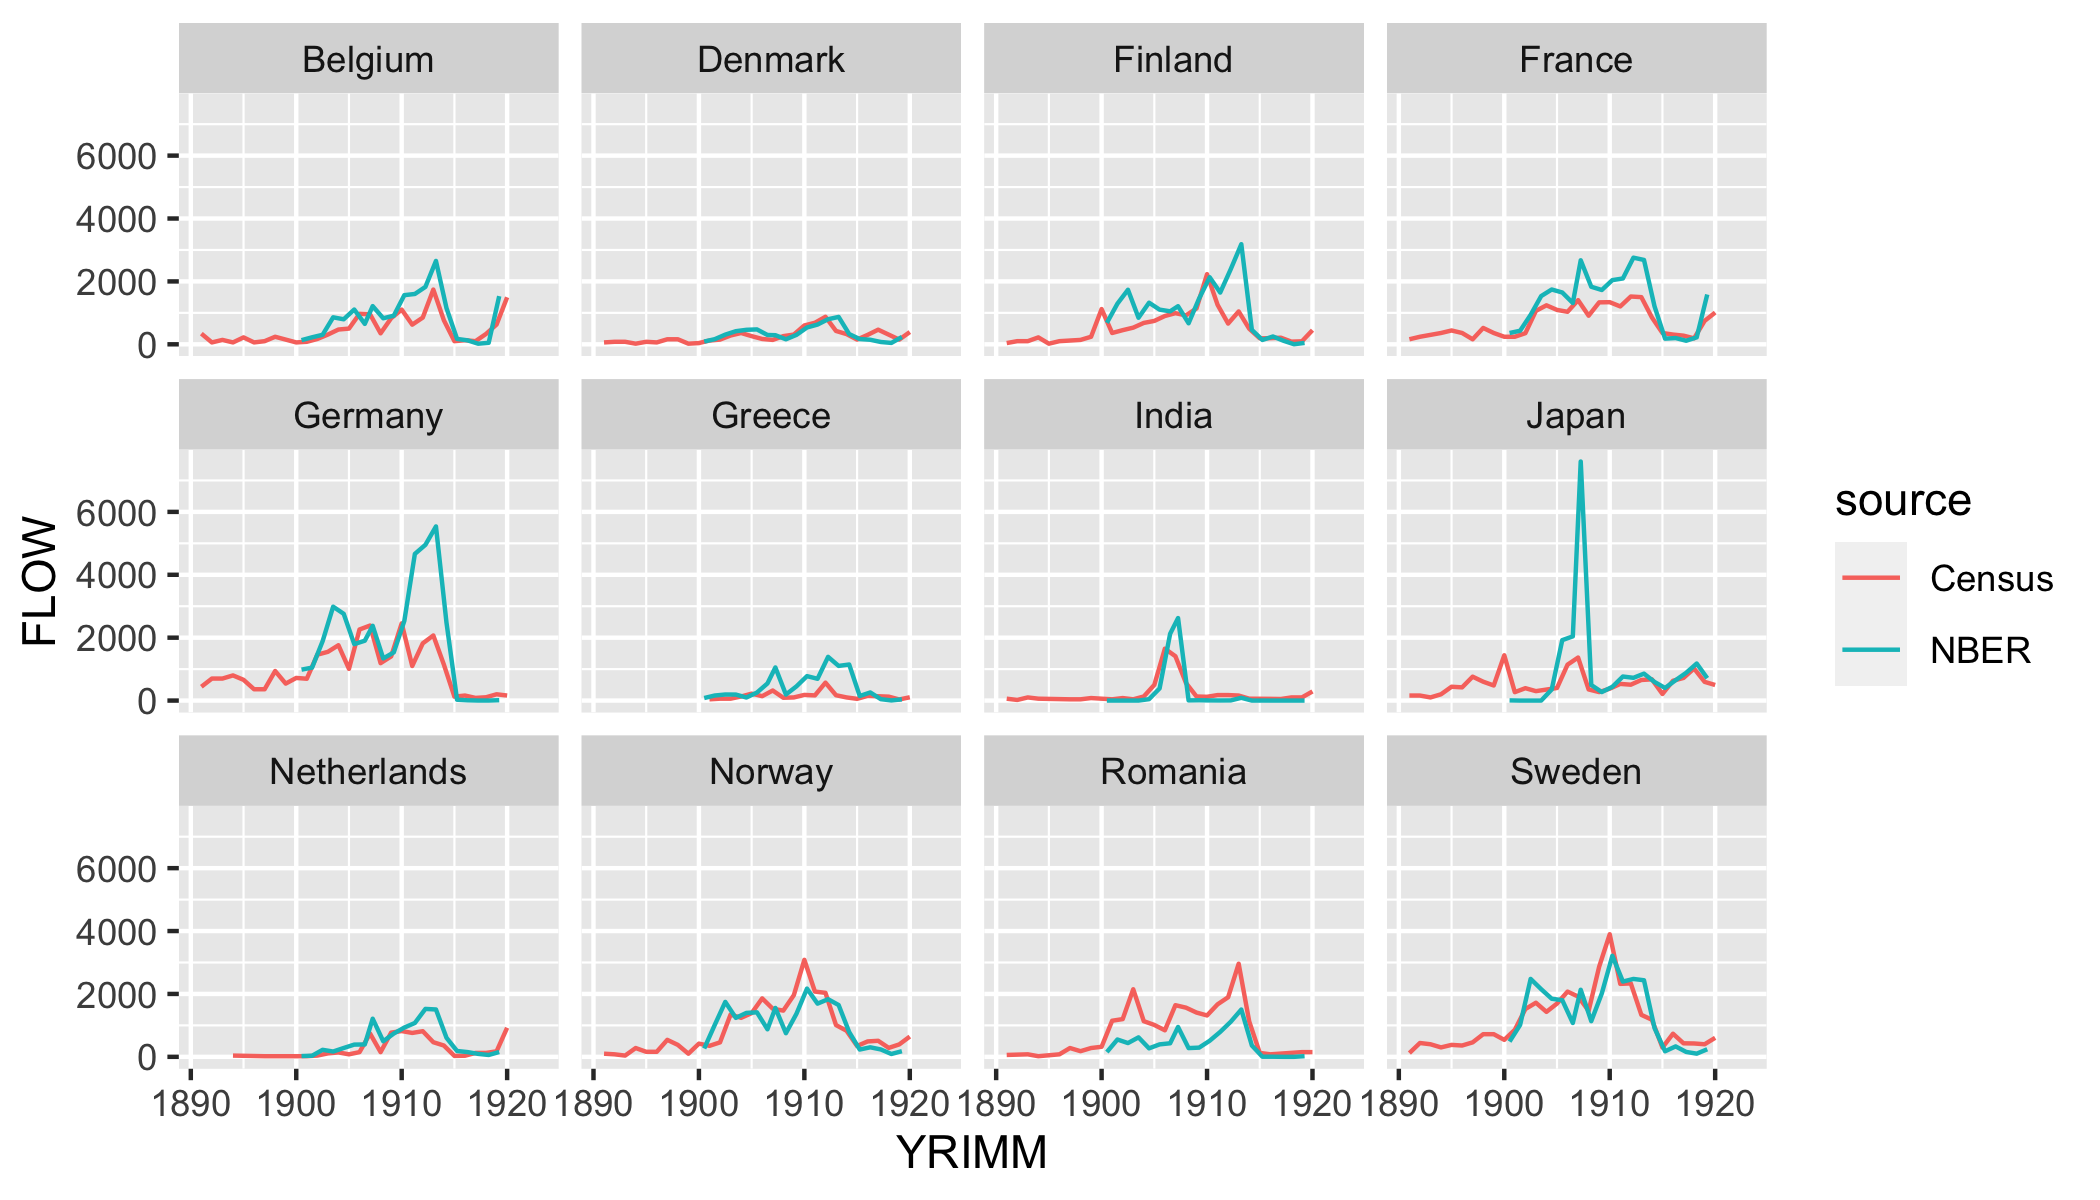
\includegraphics[width=\textwidth]{../../figs/8aug23/nber_census_compare_all.png}
		\end{center}
	\end{figure}
    \hyperlink{data1}{\beamerbutton{Back to Slides}}
\end{frame}

\begin{frame}[label = flow_compar_belgium]
	\frametitle{NBER vs. Census Immigration Data: Belgium}
    \centering
	\begin{figure}[H]
		\begin{center}
			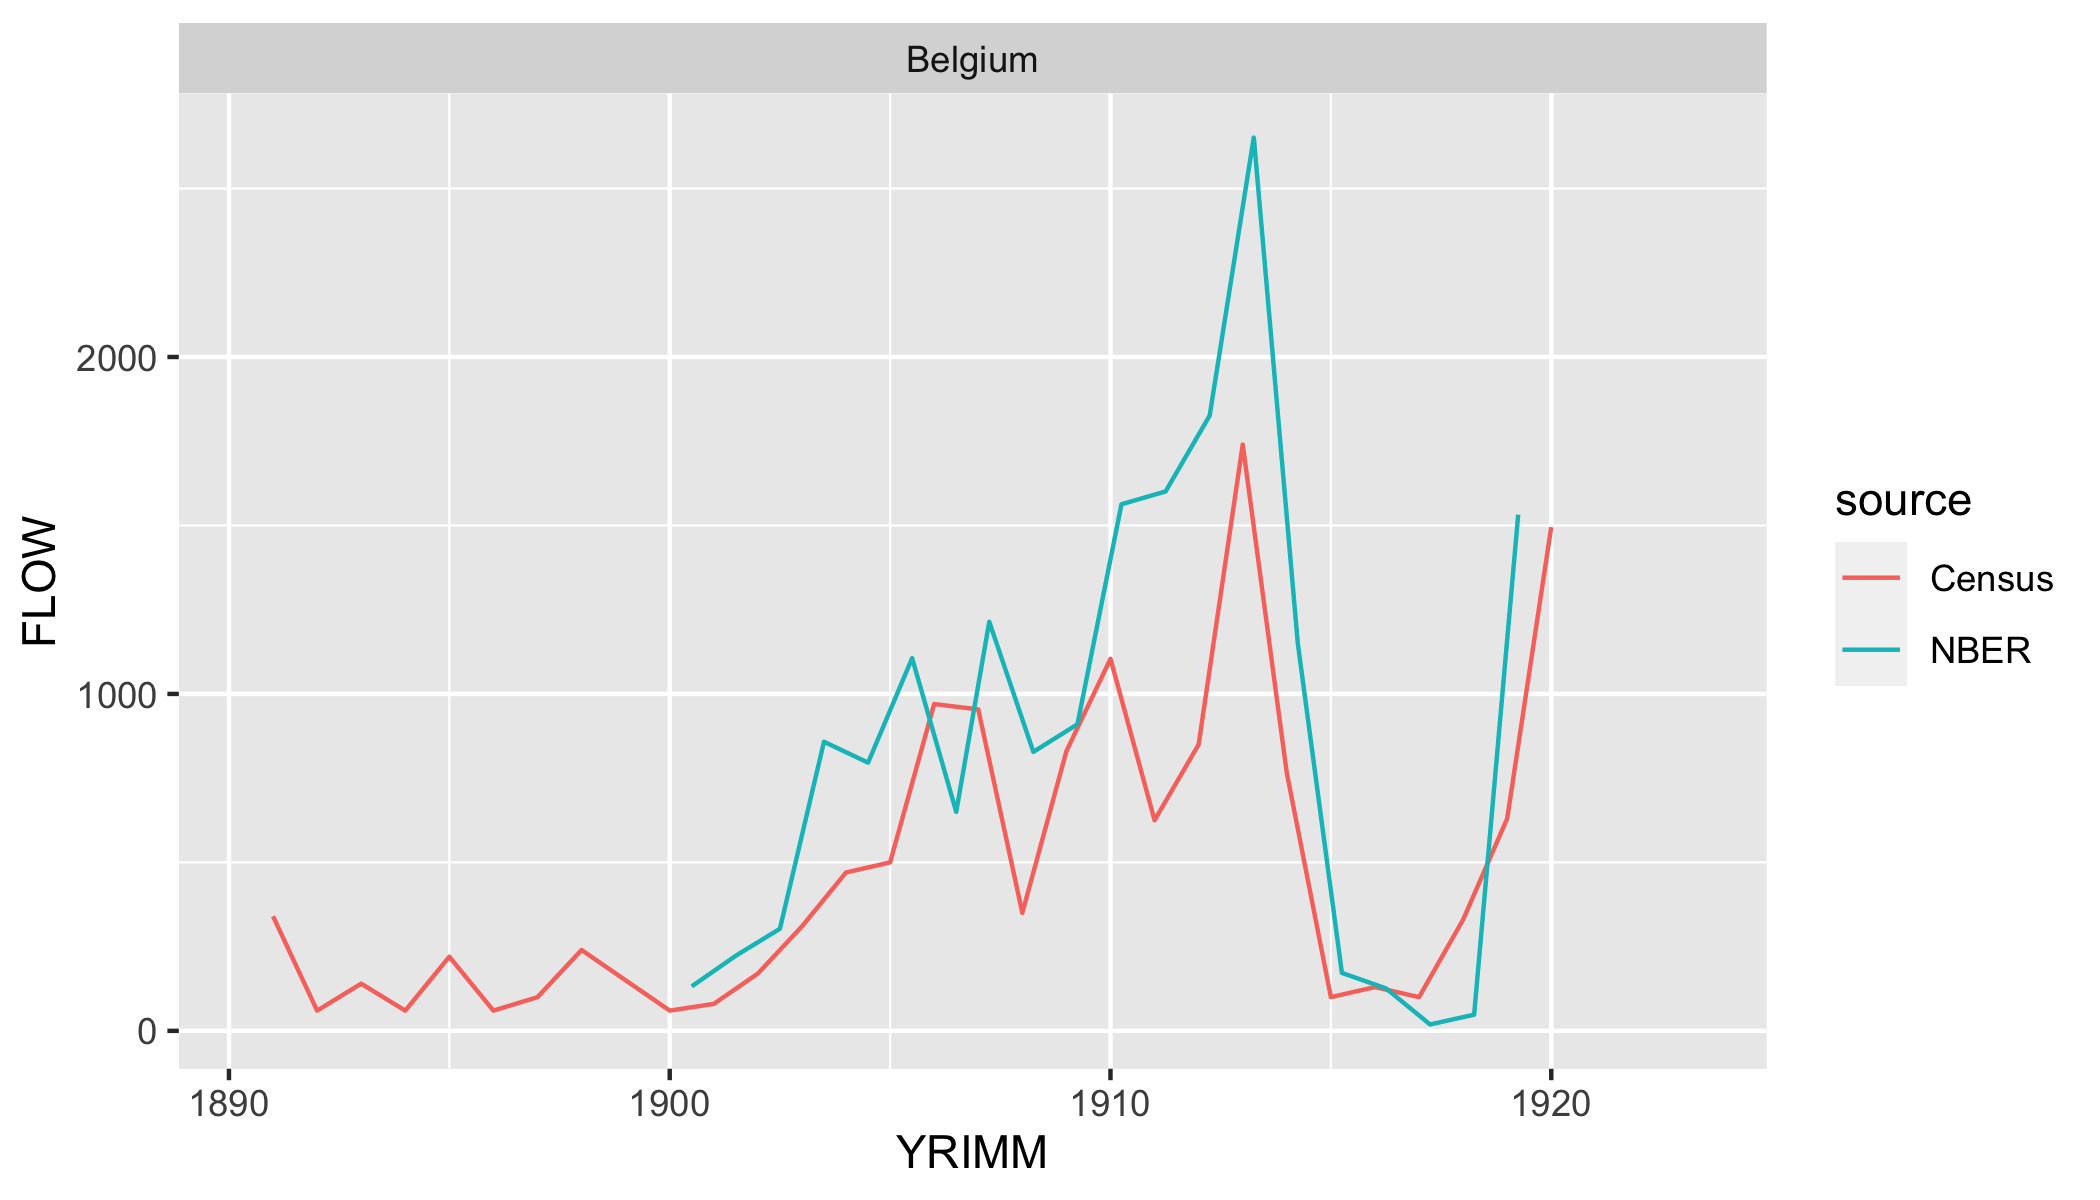
\includegraphics[width=\textwidth]{../../figs/8aug23/nber_census_compare_belgium.png}
		\end{center}
	\end{figure}
    \hyperlink{data1}{\beamerbutton{Back to Slides}}
\end{frame}


\begin{frame}[label = flow_compar_japan]
	\frametitle{NBER vs. Census Immigration Data: Japan}
    \centering
	\begin{figure}[H]
		\begin{center}
			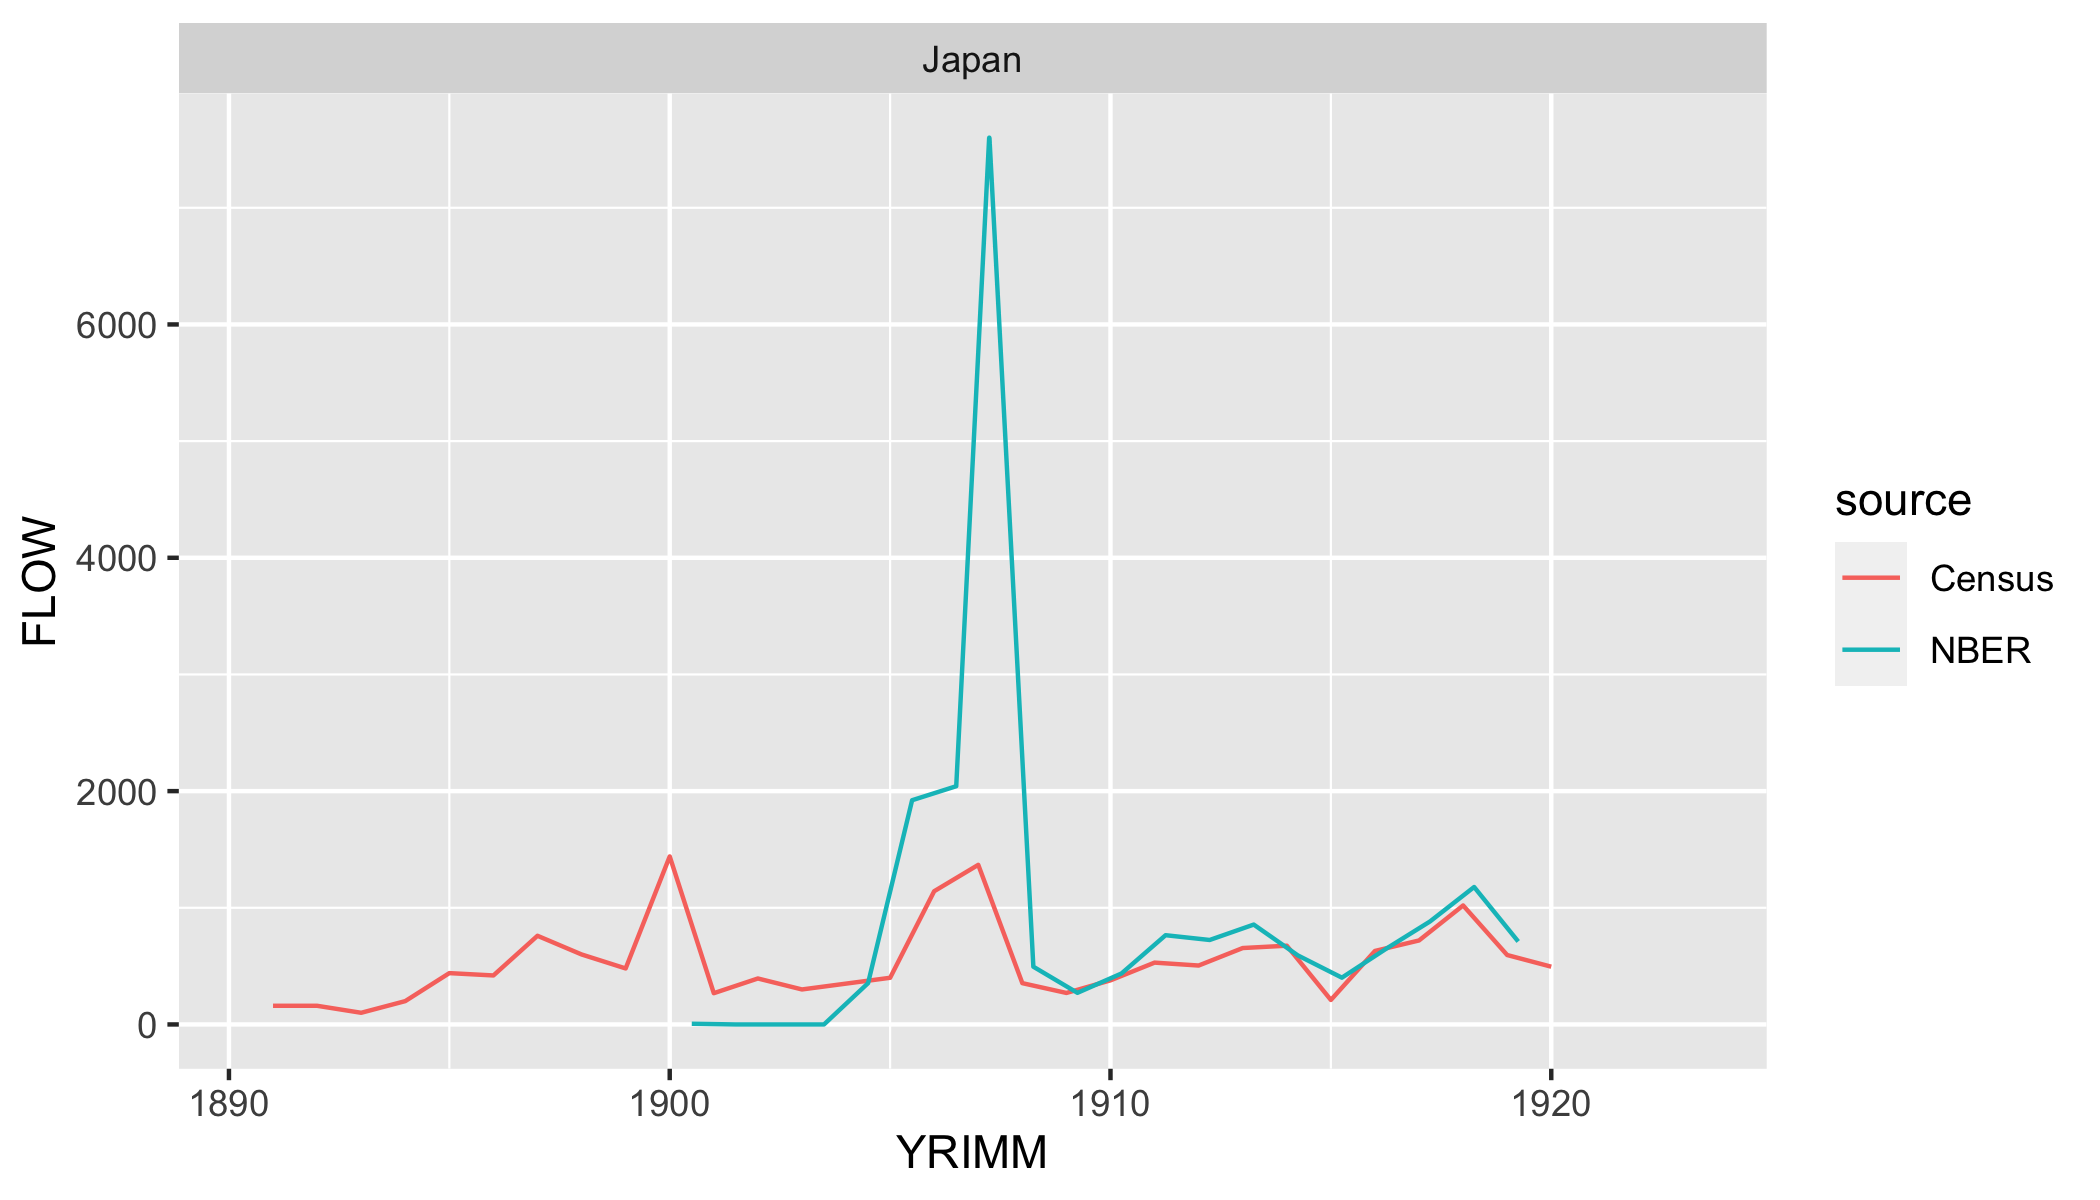
\includegraphics[width=\textwidth]{../../figs/8aug23/nber_census_compare_japan.png}
		\end{center}
	\end{figure}
    \hyperlink{data1}{\beamerbutton{Back to Slides}}
\end{frame}

\begin{frame}[label = occ_pct]
	\frametitle{Chinese Immigrant Composition: Profession at Arrival (\%)}
    \centering
	\begin{figure}[H]
		\begin{center}
			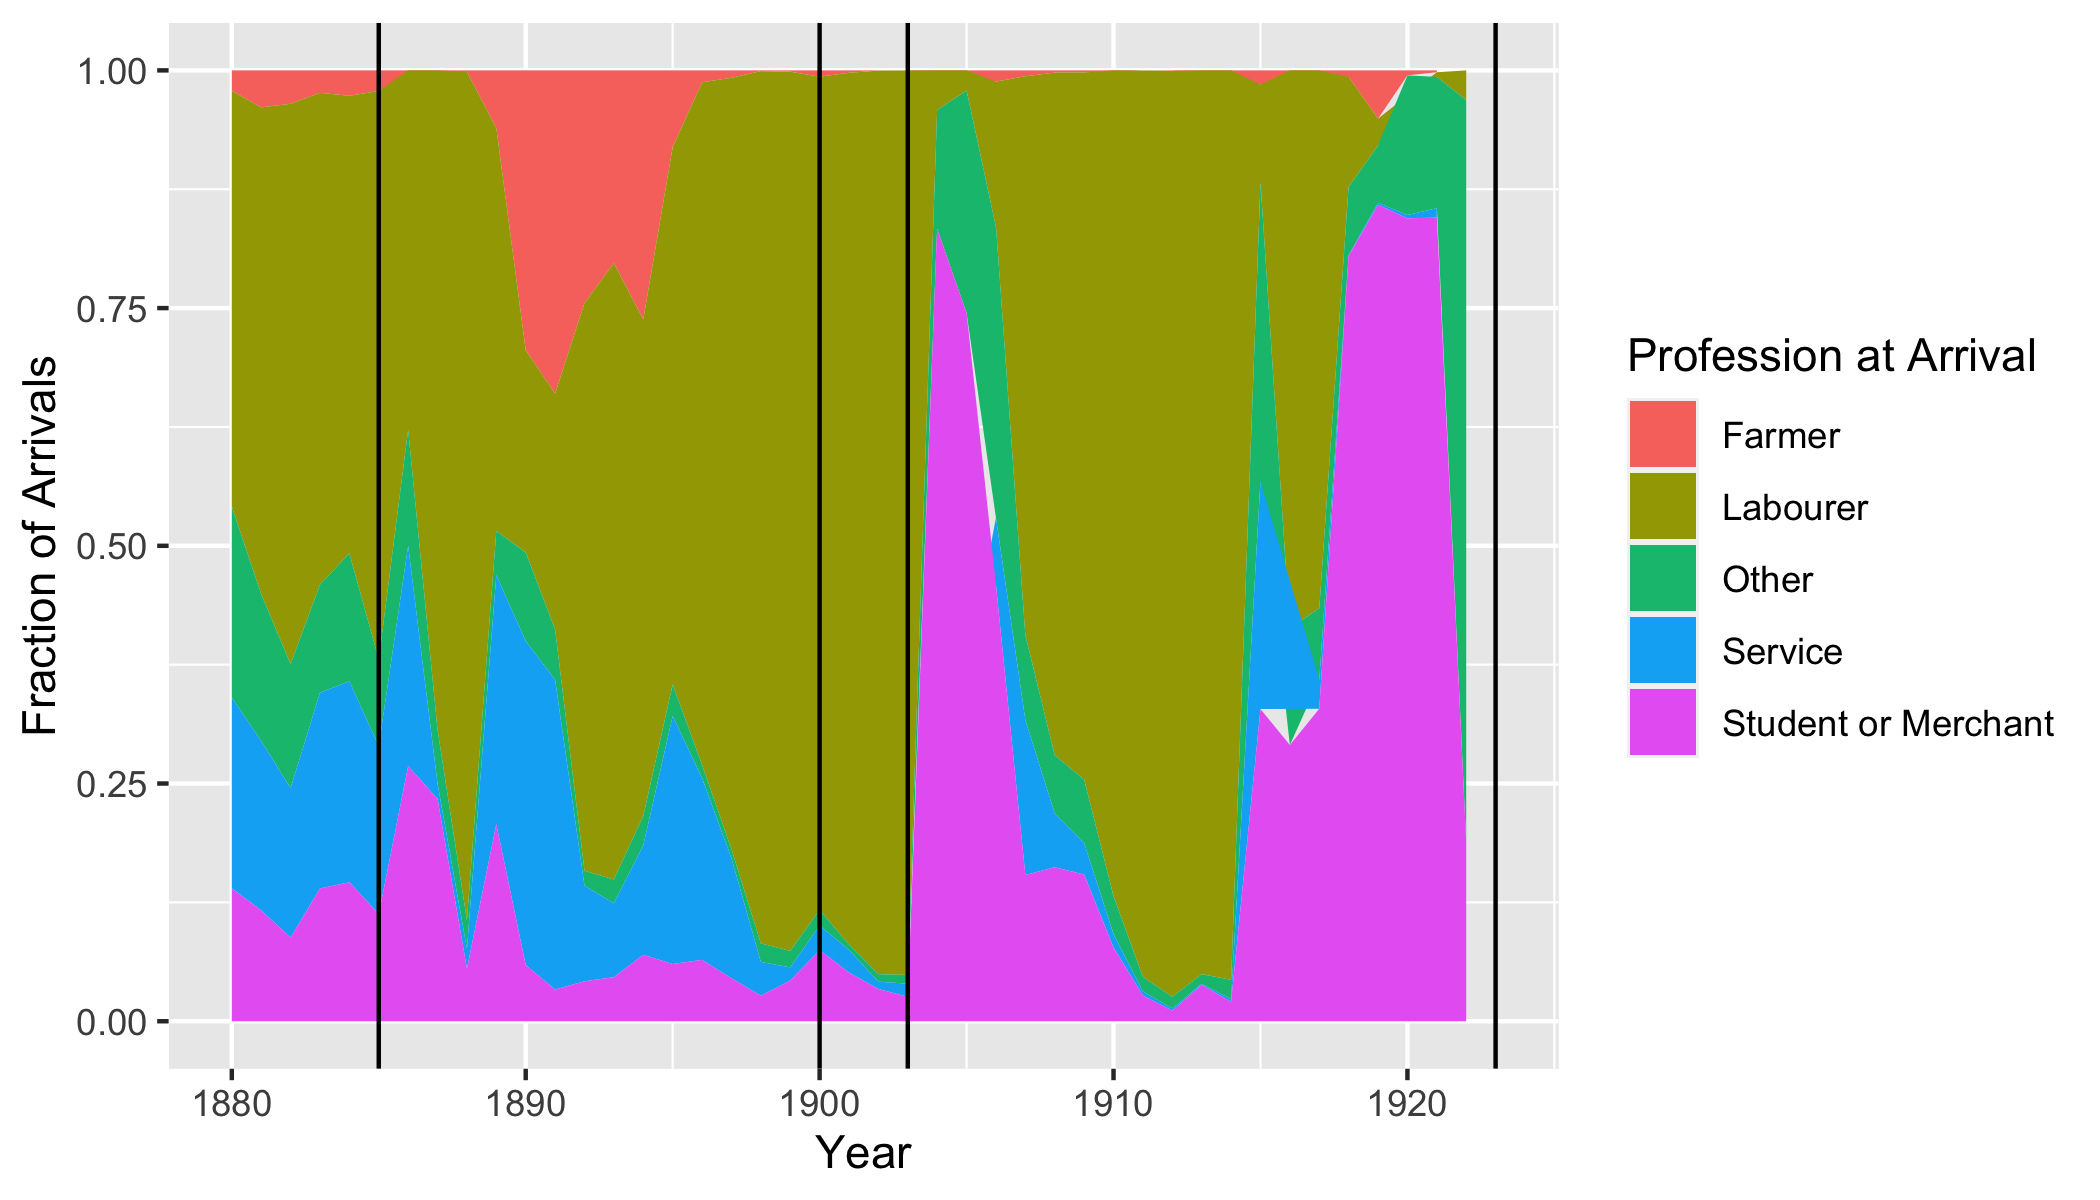
\includegraphics[width=\textwidth]{../../figs/8aug23/occgrp_pct.png}
		\end{center}
	\end{figure}
    \hyperlink{occ_n}{\beamerbutton{Back to Slides}}
\end{frame}

\begin{frame}[label = register_labor]
	\frametitle{Chinese Immigrant Composition: Laborer (\%)}
    \centering
	\begin{figure}[H]
		\begin{center}
			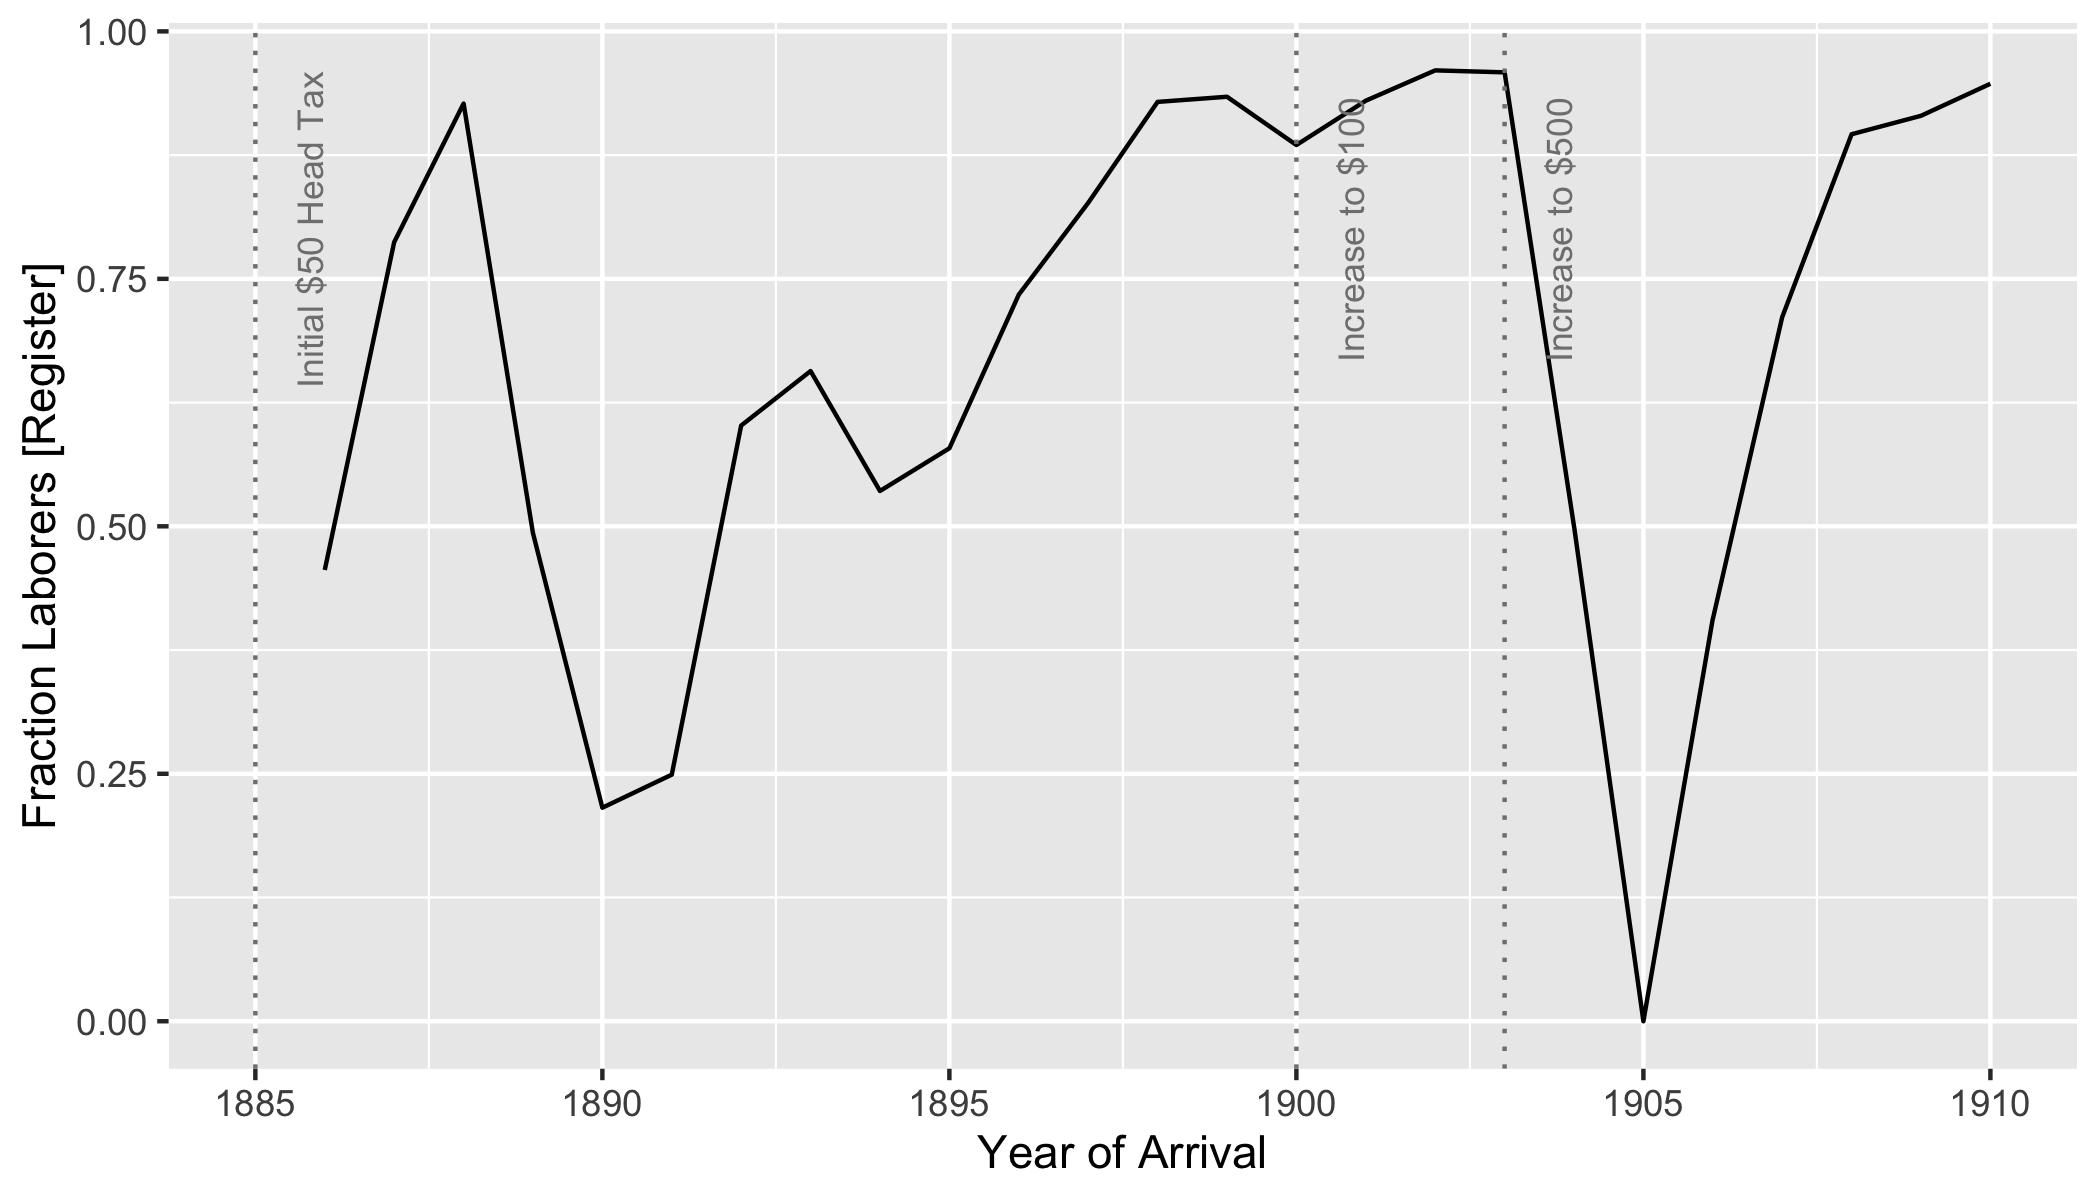
\includegraphics[width=\textwidth]{../../figs/8aug23/register_labor.png}
		\end{center}
	\end{figure}
    \hyperlink{register_regs}{\beamerbutton{Back to Slides}}
\end{frame}


\begin{frame}[label = register_height]
	\frametitle{Chinese Immigrant Composition: Avg. Height}
    \centering
	\begin{figure}[H]
		\begin{center}
			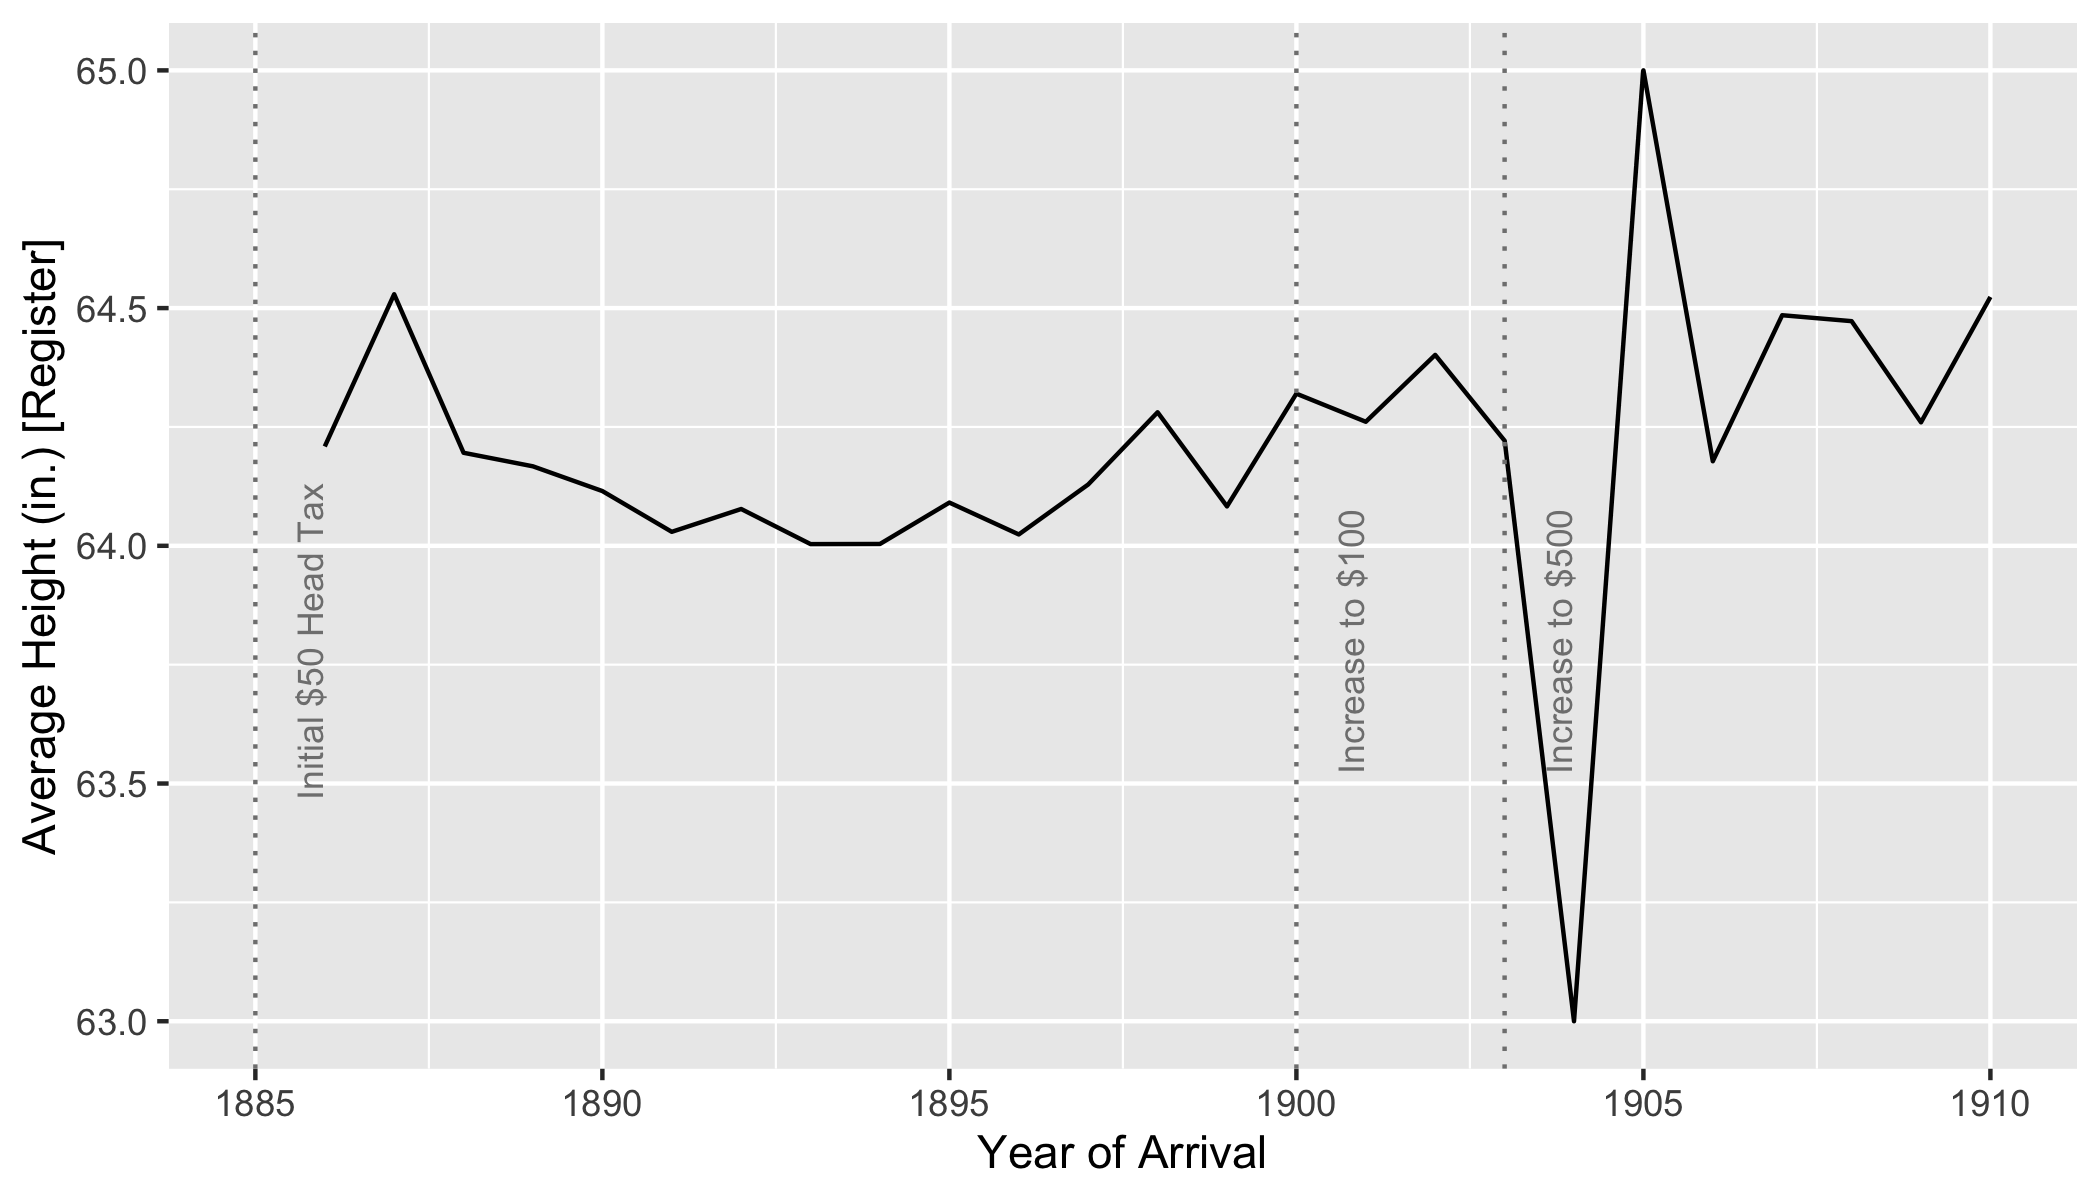
\includegraphics[width=\textwidth]{../../figs/8aug23/register_height.png}
		\end{center}
	\end{figure}
    \hyperlink{register_regs}{\beamerbutton{Back to Slides}}
\end{frame}

\begin{frame}[label = flow_us_can]
	\frametitle{Immigration Inflow: US vs. Canada}
    \centering
	\begin{figure}[H]
		\begin{center}
			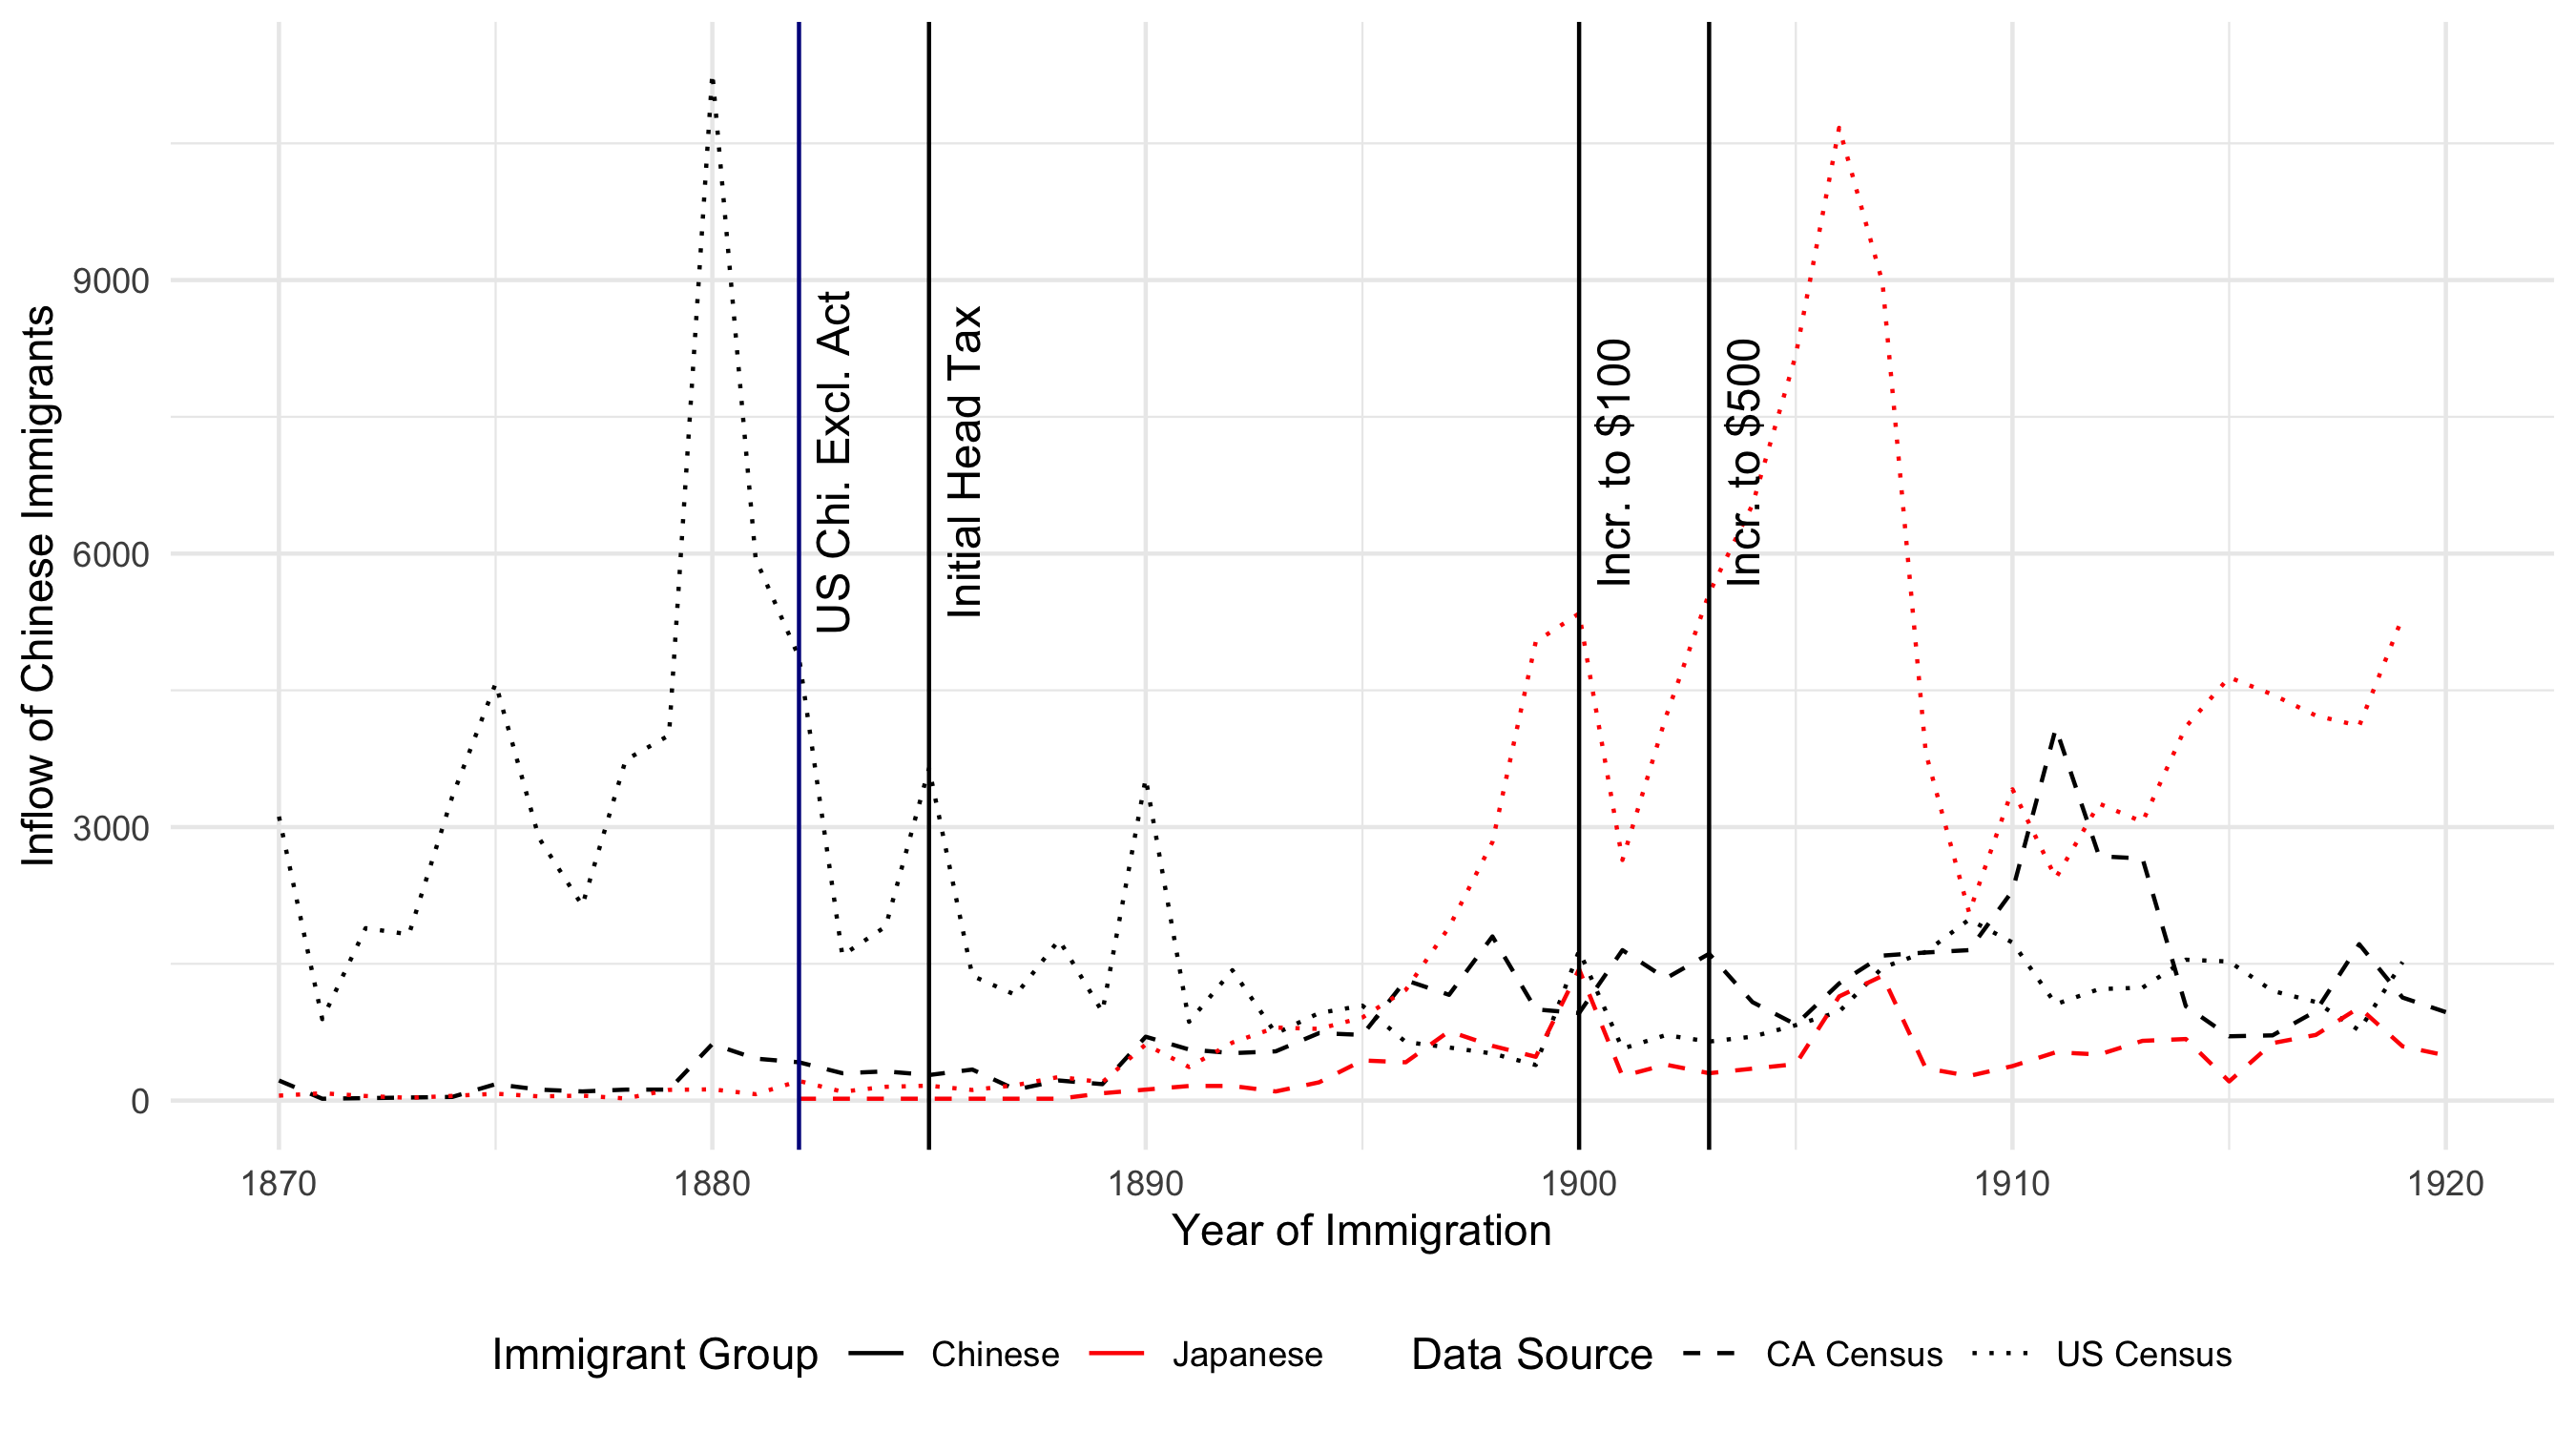
\includegraphics[width=\textwidth]{../../figs/fig3_us_can.png}
		\end{center}
	\end{figure}
    \hyperlink{reg_us}{\beamerbutton{Back to Slides}}
\end{frame}

\end{document}